\documentclass[../main.tex]{subfiles}

\begin{document}
\section{Results}\label{sec: results}
In this section we go over our results of the European Call Option and compared our result from the quantum computer to the classical result. For the Images we used this parameters $S_0 = 2, \sigma = 0.4, r=0.05, T=40/365, K=2, n=3, c=0.25$. $n$ is the number of qubits.

The European call option only depends on the price of the stock at the expiration date so we can construct the probability of the value with a log-normal distribution (described in section \ref{sec: cmc}). Qiskit has already a function to create a log-normal distribution and to load the distribution into a quantum computer. The function needs $\mu$, $\sigma_{\text{dist}}$ and lower and higher bounds to create the log-normal distribution. The result of the log-normal distribution can be seen in figure \ref{fig:E_log-normal}.
\begin{figure}[H]
  \begin{center}
    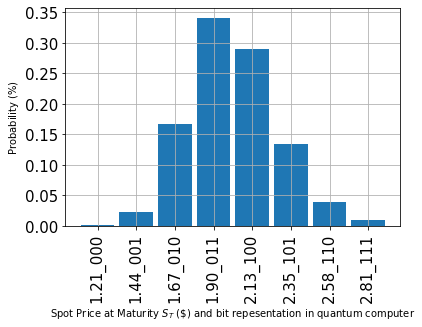
\includegraphics[width=0.5\linewidth]{../../images/probability.png}
  \end{center}
  \caption{The distinct log-normal distribution (eq. \ref{eq:lognormal}), with $\mu=(r-0.5\cdot \sigma^2)\cdot T + \log(S_0)$, $\sigma_{\text{dist}}=\sigma \cdot \sqrt{T}$ and as lower $l$ and highest $h$ value we used the 3 standard deviation. As x value the classical value is shown and the corresponding qubit state which are representing the number in our quantum computer.}
  \label{fig:E_log-normal}
\end{figure}

The equation of the European Payoff function is this
\begin{align}
    F(S(T)) = \max\{0, S(T) - K\} \label{eq:E_example_european}
\end{align}
and creates the result shown in figure \ref{fig:E_payoff_function}.
\begin{figure}[H]
  \begin{center}
    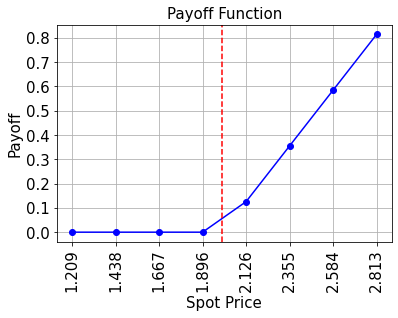
\includegraphics[width=0.5\linewidth]{../../images/payoff_european.png}
  \end{center}
  \caption{Here the value of the payoff function is shown. The breakpoints are set to $[0, 2.126]$ or $[\ket{000}, \ket{100}]$ thanks to ceil operation described in \ref{sec:MC_Payoff}}
  \label{fig:E_payoff_function}
\end{figure}

With this values we created our breakpoints, slopes and offsets. Important to know is that for our slope at breakpoint 1 we have to subtract slope(0), because the qubit already did a rotation for slope(0), the same for the offset. So we get this breakpoints, slopes and offsets, where we used $b_{\text{classic}} = [0, S_T ]$
\begin{align}
    br &= \frac{b_{\text{classic}}-l}{h-l} \cdot (2^{n}-1) \nonumber \\
    &= [0.0, 3.45206590600975] \nonumber \\
    \text{slopes}_\text{temp} &= [0, \pi c\frac{h-l}{2\cdot (f(i)_\text{max}-f(i)_\text{min}) \cdot(2^{n}-1)}] \nonumber \\
    \text{slopes}(b) &= \text{slopes}_\text{temp}(b) - \sum_{i=0}^{b-1} \text{slopes}(i) \nonumber \\
     &= [0.0,         0.22136774] \nonumber \\
    \text{offsets}_\text{temp} &= - \frac{\pi c^2}{2\cdot (f(i)_\text{max}-f(i)_\text{min})} \nonumber \\
    \text{offsets}(b) &= \text{offsets}_\text{temp} - \text{slopes}_\text{temp}(b) \cdot br(b) - \sum_{i=0}^{b-1} \text{offsets}(i) \nonumber \\
    &= [ 1.17809725, -0.76417604] \nonumber
\end{align}

This values then result in the circuit displayed in figure \ref{fig:E_model_payoff_function} and a probability distribution shown in figure \ref{fig:E_probability_estimate}
 
\begin{figure}[H]
  \begin{center}
    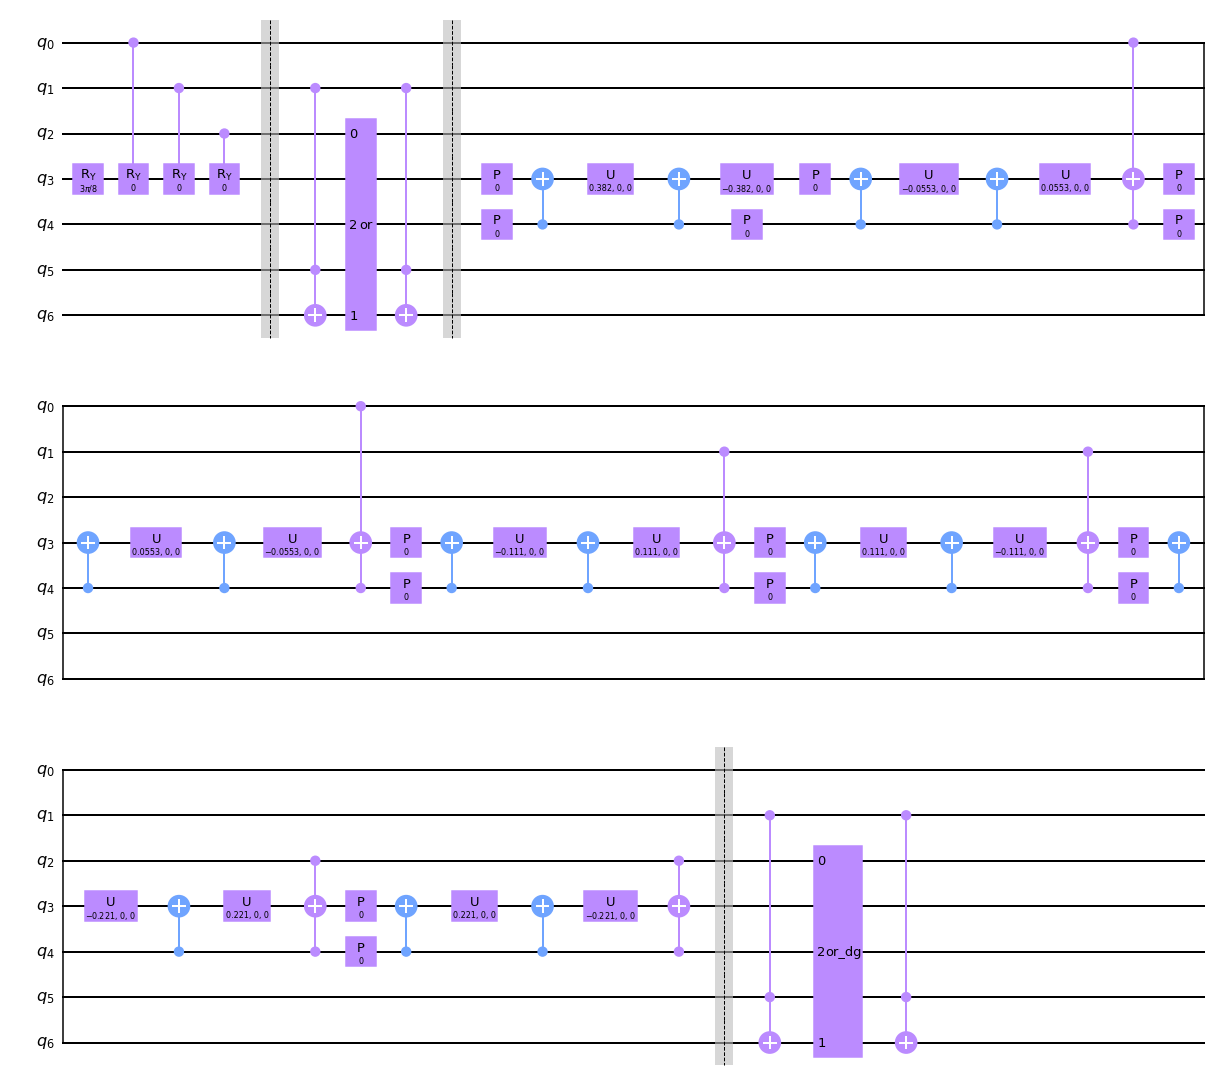
\includegraphics[width=\linewidth]{../../images/model.png}
  \end{center}
  \caption{The output of the circuit for the payoff function. The image of the circuit was generated by qiskit.\cite{Qiskit}. The circuit is divided in four sections. The first section is the $Y$-Rotation for the first breakpoint. The second section is then the greater or equal operation for the second breakpoint. The next section is then the rotation for the second breakpoint, here it good to see that the compare qubit is used to decide if the rotation should be executed or not. The last section is now the inverse of the second section.}
  \label{fig:E_model_payoff_function}
\end{figure}

 \begin{figure}[H]
  \begin{center}
    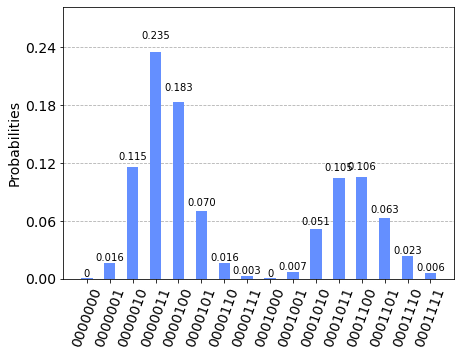
\includegraphics[width=0.5\linewidth]{../../images/probability_estimate.png}
  \end{center}
  \caption{The output after applying the payoff function to our circuit.}
  \label{fig:E_probability_estimate}
\end{figure}

The Grover Operator $\mathcal{Q}=AS_0A^\dagger S_{\psi_1}$ can now be used for the Phase Estimation Part of Amplitude Estimation. 

For European Call Options the $A$-gate of the Grover Operator is the circuit shown in figure \ref{fig:E_model_payoff_function}, $A^{\dagger}$ is simply the complex conjugate of $A$. $S_0$ is realized by a bit-flip of the objective qubit sandwiched by H-gates. The objective qubit is qubit 3 in our case, since thanks to the qubit saving implementation of $max$ function in 
\ref{fig:PF_max} a second ancilla qubit for A-gate is not needed.$S_{\psi_1} = 1-2\ket{\psi_1}\ket{0}\bra{\psi_1}\bra{0}$ is implemented using $2\ket{\psi_1}\ket{0}\bra{\psi_1}\bra{0}-1$
and a global phase bit, since the negative form can easily be implemented by using multi-controlled Z-gates sandwiched by X-gates on the target qubit. The global phase has no effect on Grovers algorithm in general. The Grover is shown in figure \ref{fig:grover}

 \begin{figure}[H]
  \begin{center}
    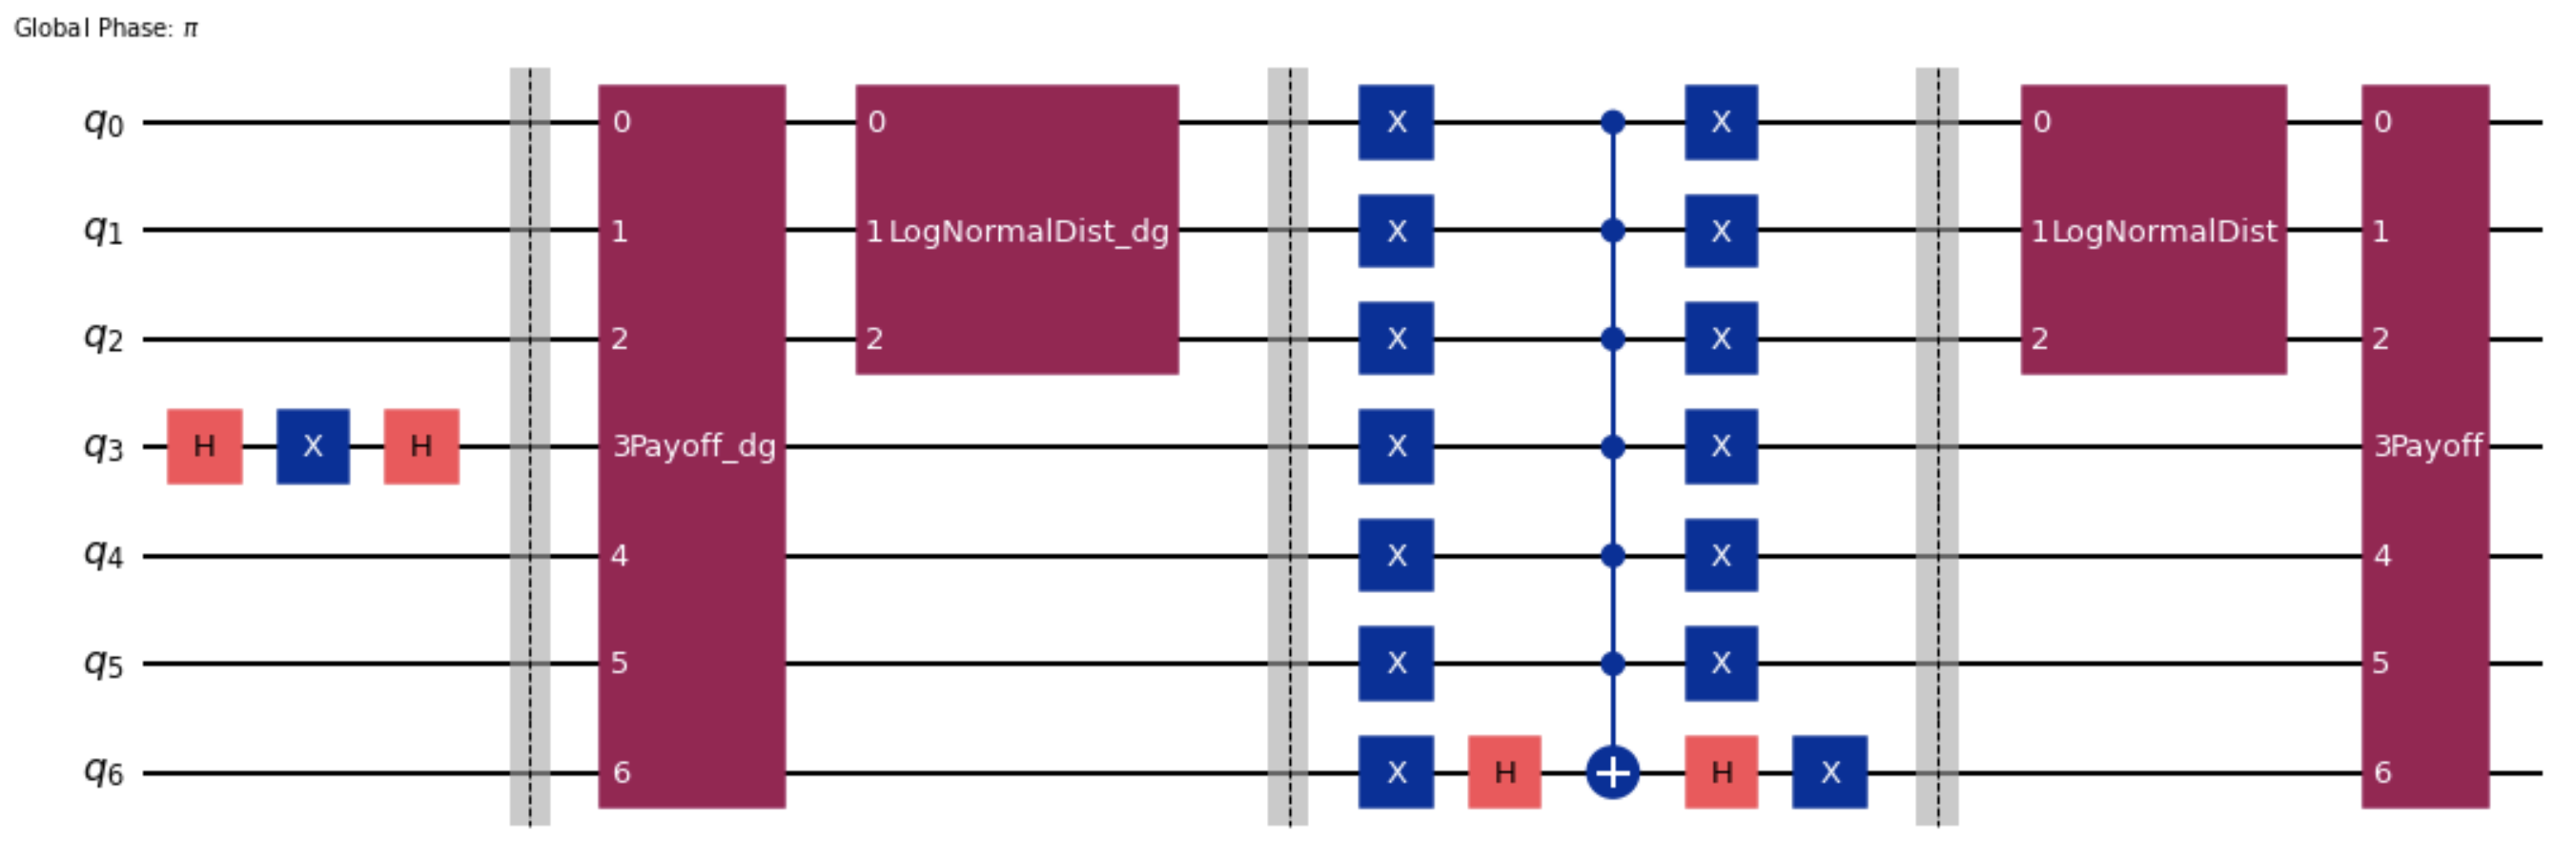
\includegraphics[width=\linewidth]{../../images/grover.png}
  \end{center}
  \caption{The Grover-operator. $S_0$ is a bit-flip implemented by a X-gate sandwiched by H-gates. $A$, $A^{\dagger}$ is the circuit and its complex-conjugate shown in figure $\ref{fig:E_model_payoff_function}$.\\
  $S_{\psi_1} = 1-2\ket{\psi_1}\ket{0}\bra{\psi_1}\bra{0}$ is implemented using $2\ket{\psi_1}\ket{0}\bra{\psi_1}\bra{0}-1$ and a global phase bit.}
  \label{fig:grover}
\end{figure}

The Grover-operator can than be applied to the first register $\ket{i}$ controlled by a second evaluation register $\ket{m}$. See figure \ref{fig:qgan} for a schematic overview.\\

 \begin{figure}[H]
  \begin{center}
    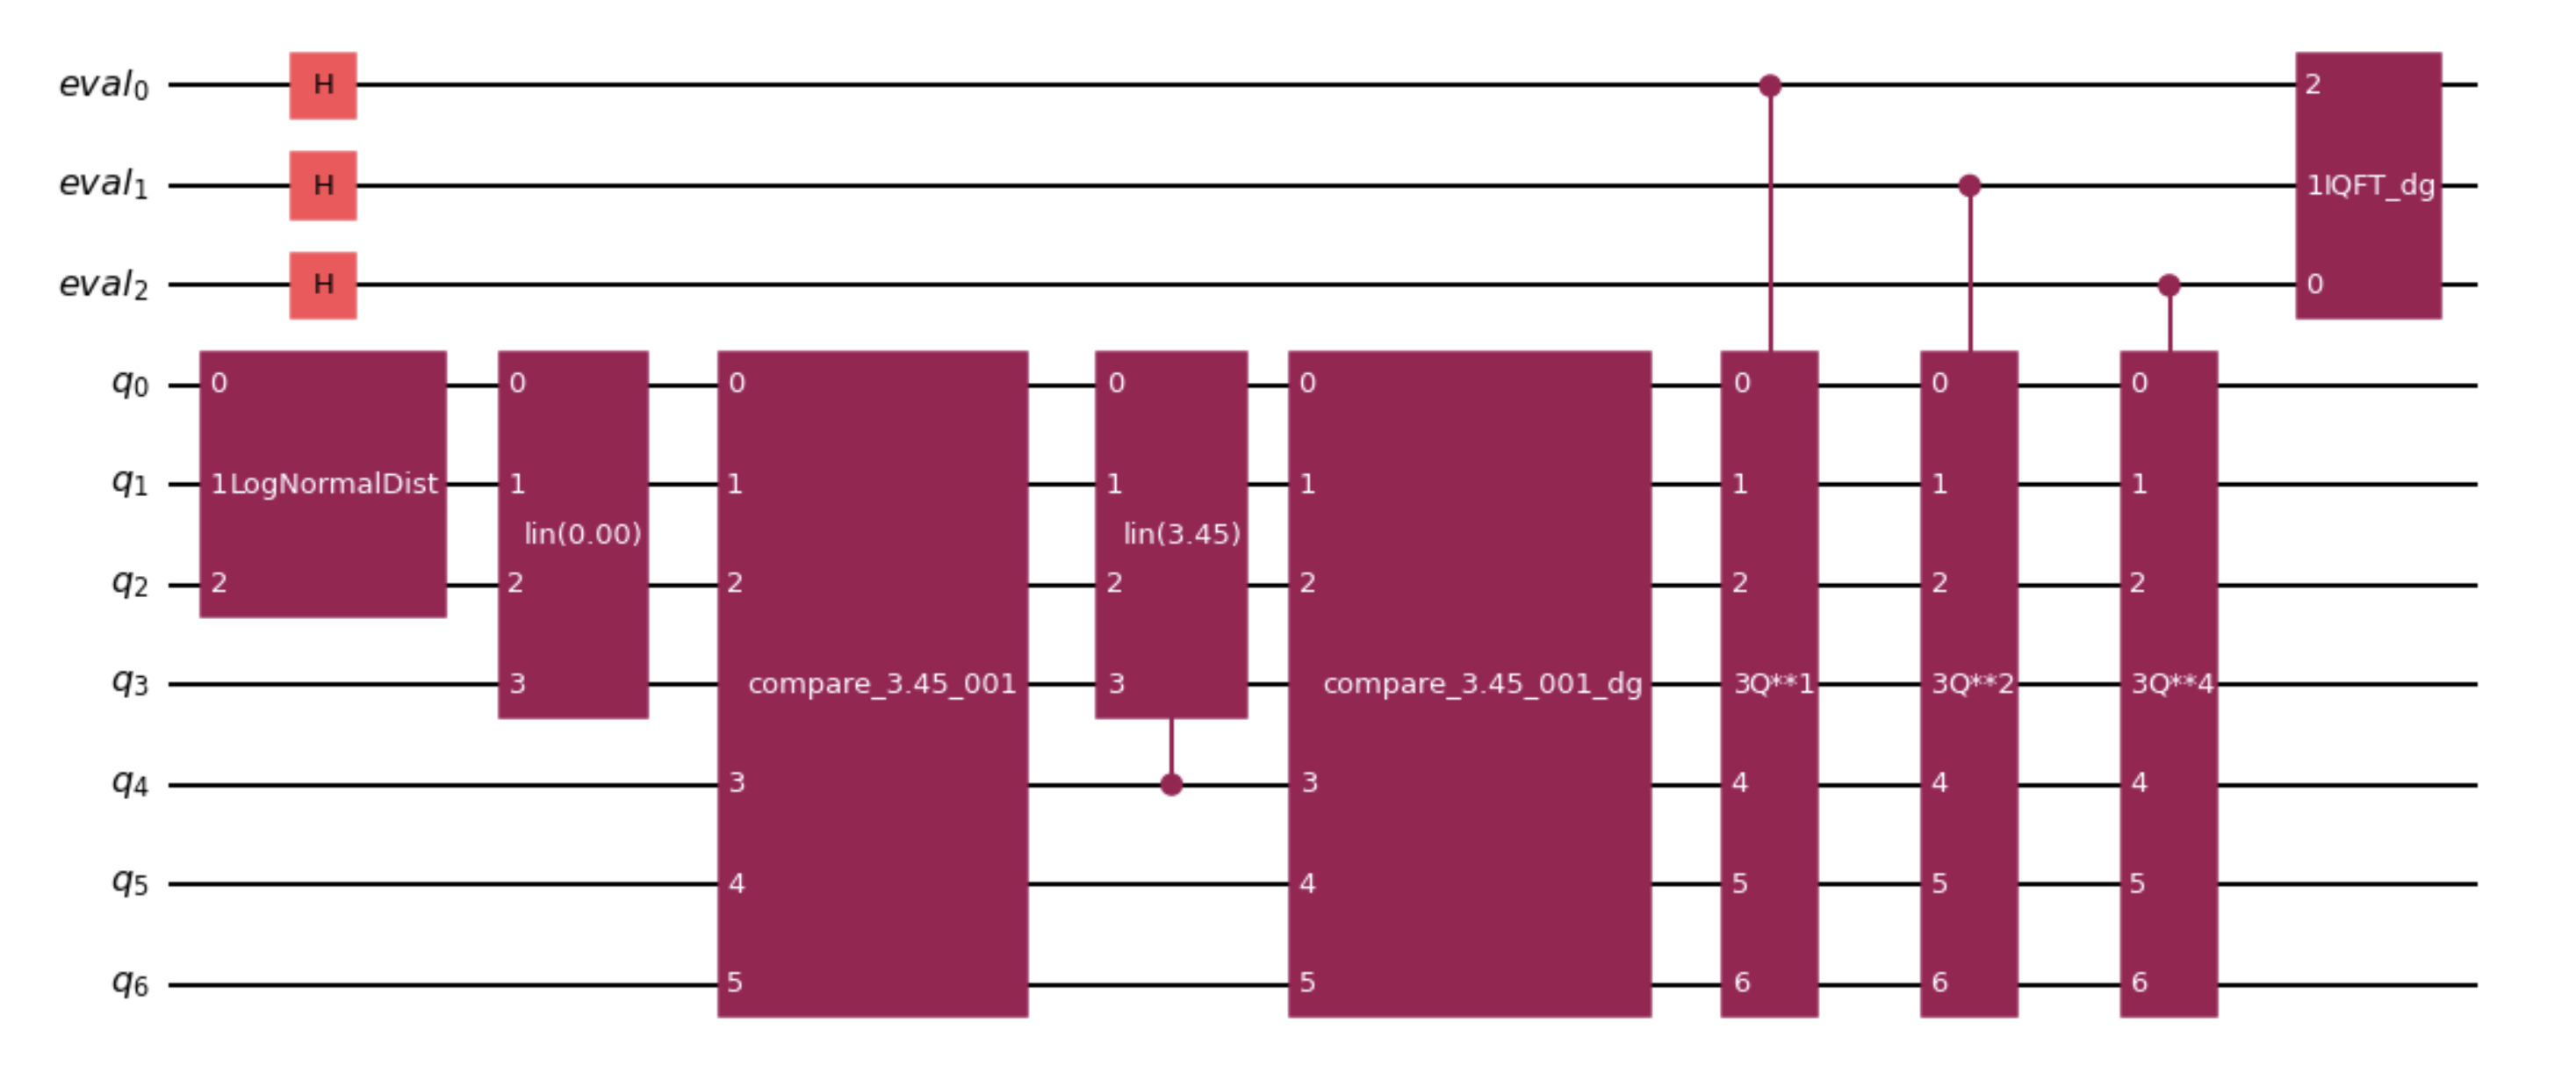
\includegraphics[width=\linewidth]{../../images/combinedCircuit.png}
  \end{center}
  \caption{The combined circuit. Note that the objective qubit here is qubit 3. Evaluation qubits are chosen for pragmatical reasons. For results a register consisting of seven qubits have been used.}
  \label{fig:combinedCircuit}
\end{figure}
The combined Circuit is displayed in figure $\ref{fig:combinedCircuit}$. For the obtained results, i.e. the estimate of Amplitude Estimation seven qubits in the evaluation register have been used. Measuring all qubits in the evaluation register gives the following result:
\begin{align}
    &\text{Exact Value: } &0.1133\\
    &\text{Estimated Value: } &0.1061\\
    &\text{95 Percent Confidence interval:	} &[0.1157, 0.1209]
\end{align}
Therefore the estimated value is close to the exact value. One problem here is that the estimated value does not lie within the confidence interval.
Note that the estimated value is the mean of applying eq. $\ref{eq:estimate_a}$ to the results of amplitude estimation. Additionally a post processing has been added in order to map from $[0,1]$ to the domain of stock prices. It is possible to apply a maximum likelihood estimator to the estimated value: 
\begin{equation}
    \text{MLE estimator value: } 0.1189.
\end{equation}
The value of the MLE estimator vaue is slightly better than the value of the ordinary estimator. Furthermore it lies within the confidence interval which is not the case for the estimated value.  
\\
 \begin{figure}[H]
  \begin{center}
    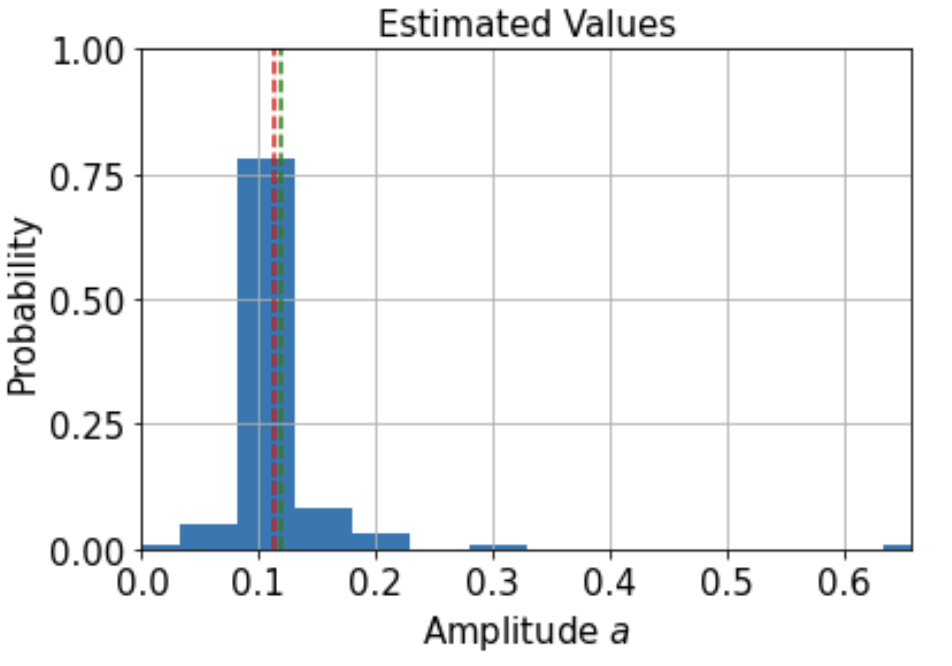
\includegraphics[width=\linewidth]{../../images/resultAE.png}
  \end{center}
  \caption{Results of Canonical AE. Red dotted line show the exact value. Green line is the MLE estimator value. }
  \label{fig:resultAE}
\end{figure}
When we now execute the same Circuit using Iterative Amplitude Estimation \cite{Grinko_2021} from qiskit we get the following results:
\begin{align}
    &\text{Exact Value: } &0.1133\\
    &\text{Estimated Value: } &0.1203\\
    &\text{95 Percent Confidence interval:	} &[0.1153, 0.1254]
\end{align}
Which is comparable to the values from Canonical Amplitude Estimation but comes with a lower cost, since Iterative Amplitude Estimation estimates the amplitude wihtout the usage of Phase Estimation and therefore with less qubits and gates.
\biblio
\end{document}